\documentclass{article}

\usepackage[utf8x]{inputenc}
\usepackage[english]{babel}
\usepackage[T1]{fontenc}
\usepackage{lmodern}
\usepackage{fullpage}
\usepackage{epstopdf}
\usepackage{graphicx}
\graphicspath{{../Images/}}
\usepackage{caption}
\usepackage{subcaption}
\usepackage{multirow}

% draw circuits
\usepackage{tikz}

% Math symbols
\usepackage{amsmath}
\usepackage{amssymb}
\usepackage{amsthm}

% Numbers and units
\usepackage{siunitx}

\usepackage[usenames,dvipsnames]{color}

\usepackage{todonotes}

\usepackage{hyperref}

\usepackage{listings}
\definecolor{gray}{rgb}{0.4,0.4,0.4}
\definecolor{dkgreen}{rgb}{0.25,0.7,0.35}
\definecolor{dkred}{rgb}{0.7,0,0} 
\lstset{language=matlab,numbers=left,numberstyle=\tiny\color{gray},basicstyle=\rm\footnotesize,keywordstyle=\bfseries\color{dkred},frame=single,commentstyle=\color{gray}=small, stringstyle=\color{dkgreen}}
% Matlab import
\usepackage{xparse}% for using parameters at the end block
\NewDocumentEnvironment{mylist}{m}{%
  \begin{#1}%
  % other code
}{%
  \end{#1}%
}

\NewDocumentEnvironment{mytable}{mm}
{\begin{table}[!ht]\centering}
{\caption{#2 Valeurs obtenues par le code du listing~\ref{lst:#1}.}\label{tab:#1}\end{table}}

\NewDocumentEnvironment{myfig}{mm}
{\begin{figure}[!ht]\centering}
{\caption{#2}\label{fig:#1}\end{figure}}
\NewDocumentEnvironment{myfigsub}{mmm}
{\begin{subfigure}[b]{#3\textwidth}}
{\caption{#2}\label{fig:#1}\end{subfigure}}

\newcommand{\mysubfig}[3]
{\begin{myfigsub}{#1}{#2}{#3}
    \includegraphics[width=\textwidth]{#1.png}
\end{myfigsub}}
\newcommand{\mysubfigg}[4]
{\begin{myfigsub}{#1}{#2}{#3}
    \includegraphics[#4, width=\textwidth]{#1.png}
\end{myfigsub}}


\newcommand{\myfullfig}[3]
{\begin{figure}[!ht]
    \centering
    \includegraphics[width=#3\textwidth]{#1.png}
    \caption{#2}
    \label{fig:#1}
\end{figure}}


\newcommand{\matlabplot}[2]
{\begin{figure}[!ht]\centering
\includegraphics[width=\textwidth]{img/#1.png}
\caption{#2 Graphique obtenu par le code du listing~\ref{lst:#1}.}\label{fig:#1}\end{figure}}


\newcommand{\matlabcode}[2]
{\lstinputlisting[caption={Contenu du fichier \lstinline{#1.m}
  contenant l'implémentation de la fonction \lstinline{#1}.
#2},label={lst:#1}]
{../matlab/#1.m}
}



\DeclareMathOperator{\newdiff}{d} % use \dif instead
\newcommand{\dif}{\newdiff\!}
\newcommand{\fpart}[2]{\frac{\partial #1}{\partial #2}}
\newcommand{\ffpart}[2]{\frac{\partial^2 #1}{\partial #2^2}}
\newcommand{\fdpart}[3]{\frac{\partial^2 #1}{\partial #2\partial #3}}
\newcommand{\fdif}[2]{\frac{\dif #1}{\dif #2}}
\newcommand{\ffdif}[2]{\frac{\dif^2 #1}{\dif #2^2}}
\newcommand{\constant}{\ensuremath{\mathrm{cst}}}
\newcommand{\rha}{\hat{r}^n_{MLE}}
\newcommand{\bigoh}{\mathcal{O}}
\newcommand{\F}{\mathcal{F}}

\DeclareMathOperator{\pois}{Pois}
\DeclareMathOperator{\sinc}{sinc}
\DeclareMathOperator{\var}{Var}
\DeclareMathOperator{\argmax}{argmax}

\usepackage{parskip} % Ajoute de l'espace entre les paragraphes et mets l'indentation to 0
\setlength{\parindent}{15pt} % Remets l'indentation par default

\newcommand{\figref}[1]{figure~\ref{fig:#1}}


%\includeonly{Chapters/train}
\title{ \textbf{Erratum Complexity} \\ - Project of picture deblurring - }
\author{Jonathan \textsc{Berthe} \and Arnaud \textsc{Cerckel} \and Benoît \textsc{Legat} \and Geoffroy \textsc{Vanderrreydt}}
%\institute{LFSAB1507}
\begin{document}

\maketitle

\subsection{Complexity of our different results}


As done in the report, let's estimate the complexity of the deconvolution algorithms. To do so, we use the same picture. We first deblur the picture using \texttt{deconvlucy} for a certain size($125 \times 125$ here), then for $250 \times 250$, until $2500 \times 2500$ (the original picture  size was $5184 \times 3456$) with each time 16 iterations of Lucy. Afterwards we compute  \texttt{deconvwnr} and \texttt{deconvreg} in the same way. The figure \ref{fig:ComplexityRelbw} plots the ratio ``time needed to compute the picture/ time needed to compute the smallest picture'' on the y axis and on the x axis the ratio ``number of pixels of the picture / number of pixels of the smallest picture''. We see that as the number of pixels rises by 400, the time needed to compute rises by around 800 for Lucy and by around 100 for the two other algorithms. So \texttt{deconvlucy} is clearly slower than the two others. 


\begin{figure}[h!]
\centering
\begin{subfigure}{0.4\textwidth}
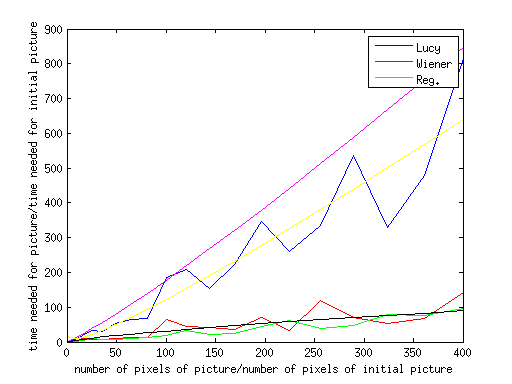
\includegraphics[{width= \textwidth}]{../Images/ComplexityRelbw.png}
\caption{The ratio ``time needed to compute the picture/ time needed to compute the smallest picture'' is the y axis and the x axis is the ratio ``number of pixels of the picture / number of pixels of the smallest picture''.}
\label{fig:ComplexityRelbw}
\end{subfigure}
~
\begin{subfigure}{0.4\textwidth}
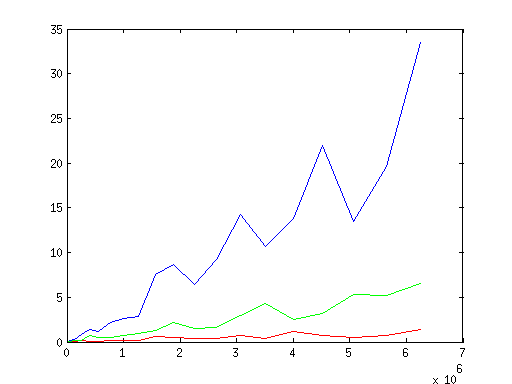
\includegraphics[{width= \textwidth}]{../Images/ComplexityAbsbw.png}
\caption{Time  needed to compute the picture on the y-axis, number of pixels of the picture on the x-axis.}
\label{fig:ComplexityAbsbw}
\end{subfigure}
\caption{Complexity of our different algorithms for a black and white picture. The blue line is for \texttt{deconvLucy}, the red one for \texttt{deconvwnr} and the green one for \texttt{deconvreg}.}
\label{fig:Complexity}
\end{figure}

If we have a quick look to color image which means $125 \times 125 \times 3$ pixels, $250 \times 250 \times 3$ etc., we see that the relative time needed is almost the same which is is logical, figure~\ref{fig:ComplexityRel}. As regards the absolute time needed to compute the image, we needed for the biggest picture around $33$ seconds for Lucy, $5$ seconds for Regularisation and $1.5$ seconds for Wiener, figure~\ref{fig:ComplexityAbsbw}; we are now around $100$, $18$ and $4$ seconds, figure~\ref{fig:ComplexityAbs}. This result makes sense. Indeed, with Lucy when it's a color picture it's simply a loop for each color, so 3 times more time required. We can reasonably suppose that the two others algorithms use the same process.


\begin{figure}[h!]
\centering
\begin{subfigure}{0.4\textwidth}
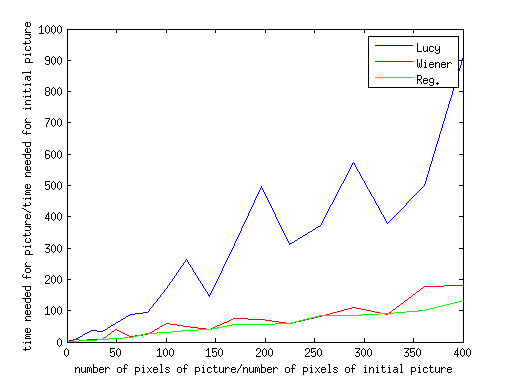
\includegraphics[{width= \textwidth}]{../Images/ComplexityRel.png}
\caption{The ratio ``time needed to compute the picture/ time needed to compute the smallest picture'' is the y axis and the x axis is the ratio ``number of pixels of the picture / number of pixels of the smallest picture''.}
\label{fig:ComplexityRel}
\end{subfigure}
~
\begin{subfigure}{0.4\textwidth}
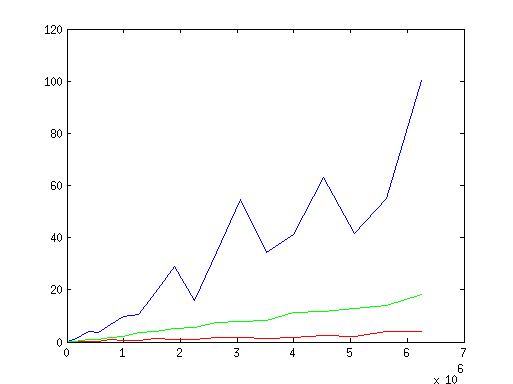
\includegraphics[{width= \textwidth}]{../Images/ComplexityAbs.png}
\caption{Time  needed to compute the picture on the y-axis, number of pixels of the picture on the x-axis.}
\label{fig:ComplexityAbs}
\end{subfigure}
\caption{Complexity of our different algorithms for a color picture. The blue line is for \texttt{deconvLucy}, the red one for \texttt{deconvwnr} and the green one for \texttt{deconvreg}.}
\label{fig:Complexity}
\end{figure}



Let's now have a look at the complexity of our \texttt{robust\_angle\_estimator} method. Proceeding in the same way as for the deconvolution algorithms, we generate the plot shown in figure \ref{fig:ComplexityRadon}. Now the results are far more logical than in the report. Indeed the relation between time and number of pixels is linear. If we have to deal with 400 times more pixels than at the beginning we can expect 400 times more time needed than at the beginning. 


\begin{figure}[h!]
\centering
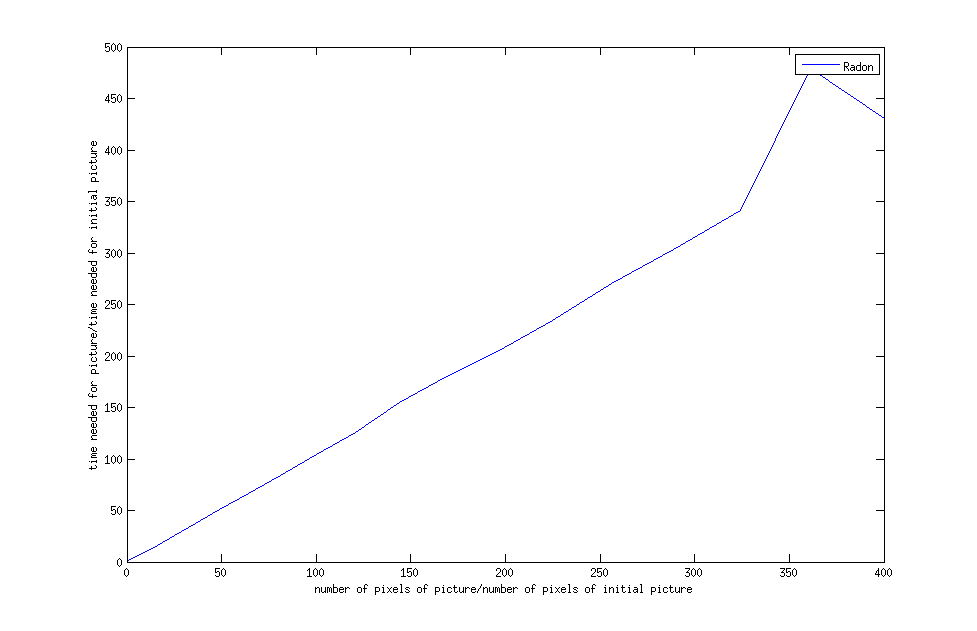
\includegraphics[scale=0.4]{../Images/ComplexityRadon.png}
\caption{Complexity of our \texttt{robust\_angle\_estimator} method}
\label{fig:ComplexityRadon}
\end{figure}






\end{document}
